\documentclass[./main.tex]{subfiles}
\begin{document}
\chapter{微积分观点下的曲线与曲面}
从观摩Euclid写就\textit{Elements}, 到目睹Apollonius完成\textit{Conics}, 你已经历许多. 但是仅仅凭借初等数学的工具, 你的前进变得越发困难. 是时候引入强大的分析思想裁弯取直, 使用线性代数的丰富工具, 驯服那令人胆寒的曲线曲面.
\section{分析思想能带来什么}
建立直角坐标系的过程中, 我们将\(\mathbb{E}^3\)等同于\(\mathbb{R}^3\). 点变成了三个一组的实数, 意味着Euclid空间连续、平直等特性通过实数的公理得到了阐释.

曲线变成了数组的一维集合, 而值得我们研究 (性质足够好) 的曲线, 则对应连续可微向量值函数的像集. 之所以以连续可微作为``性质够好''的标准, 是因为在我们的常识里, 曲线应当具有``方向''``长度''等基本的属性, 这些属性能被``良好地定义'', 就要求连续可微. 另外, ``曲率''等更高级的性质还需要更高阶的可导. 不过不用担心, 目前只需要接触任意阶可导的曲线, 它们有好听的名字——光滑曲线.

曲面只是二维的推广, 光滑目前看是一个普遍满足的要求, 因此可以赋予``方向''``曲率''``度量''\marginpar{\footnotesize 度量提供了长度.}等属性. 由于曲面是一个比曲线更丰富有趣的对象, 并且作为二维对象仍处于能运用几何直观的范围, 对于曲面的研究是我们当下的重点.
\section{曲线的分析化}
将曲线用向量值函数表示的方式一定是不唯一的, 只需要这些函数的值域相同即可. 但是对于一条曲线, 我们总是倾向于选择性质最好的一种表示. 就一般情况而言, 满足
\[
    \left|\mathbf{r}'(t)\right|=1,\quad\forall t\in I
\]
的曲线表示\(\mathbf{r}(t),\ t\in I\), 也就是每个点处的切向量都是单位切向量的表示, 在``长度''``曲率'' 这几个量的定义上比较简洁.
\subsection{长度}\label{sec:2}
我们一般会用折线段长度的极限作为原来曲线的长度. 对一条曲线\(\mathbf{r}(t),t\in I\), 用其上\(n+1\)个点\(\mathbf{r}(x_0),\mathbf{r}(x_1),\dots\mathbf{r}(x_n)\)分割, 其中\(\inf I=x_0<x_1<\cdots<x_{n-1}<x_n=\sup I\).

\begin{figure}[!ht]
    \centering
    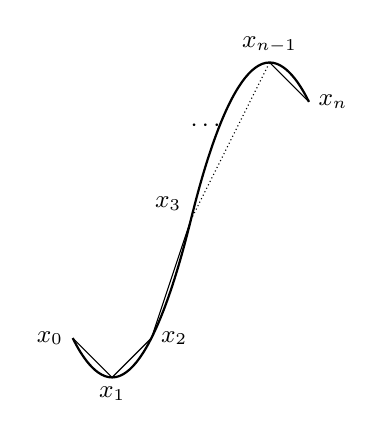
\begin{tikzpicture}
        \draw[thick] (0,0) parabola bend (0.5,-0.5) (1.5,1.5);
        \draw[thick] (1.5,1.5) parabola bend (2.5,3.5) (3,3);
        \draw (0,0) node[left]{\small\(x_0\)} -- (0.5,-0.5) node[below]{\small\(x_1\)} -- (1,0) node[right]{\small\(x_2\)} -- (1.5,1.5) node[above left]{\small\(x_3\)};
        \draw[densely dotted] (1.5,1.5) -- node[above left]{\small\(\cdots\)} (2.5,3.5);
        \draw (2.5,3.5) node[above]{\small\(x_{n-1}\)} -- (3,3) node[right]{\small\(x_n\)};
    \end{tikzpicture}
\end{figure}
于是得到了一个拟合的表达式
\begin{equation}\label{equ:1}
    s\approx\sum_{i=1}^n |\mathbf{r}(x_i)-\mathbf{r}(x_{i-1})|\approx\sum_{i=1}^n |\mathbf{r}'(x_i)(x_i-x_{i-1})|=\sum_{i=1}^n |\mathbf{r}'(\xi_i)|(x_i-x_{i-1}).
\end{equation}
第二个\(\approx\)是因为在\(x_{i-1},x_i\)十分接近的时候, 可以将\(\mathbf{r}(x_i)-\mathbf{r}(x_{i-1})\)近似为\(\mathbf{r}'(x_i)(x_i-x_{i-1})\). 发现\eqref{equ:1}最右边是一个Riemann和,所以对\eqref{equ:1}两边取极限就得到\marginpar{\footnotesize 这就是讲义里弧长定义的直观解释.}
\begin{equation}\label{equ:2}
    s=\int_{x_0}^{x_n}|\mathbf{r}'(x)|\dd x.
\end{equation}
对于曲线参数化定义域里的每个区间, 都有对应曲线段的长度, 而由于定积分的可加性, 可以固定区间的起点为\(t_0\).
\[
    s(I)=\int_I|\mathbf{r}'(x)|\dd x\qquad\longrightarrow\qquad s(t)=\int_{t_0}^t|\mathbf{r}'(x)|\dd x,
\]
那么对于端点为\(a\)和\(b\)的区间, 对应的曲线长度就是\(|s(b)-s(a)|\).

回到弧长参数化, 我们发现, 在\(|\mathbf{r}'(t)|\equiv1\)的约定下, \(s(t)=\int_{t_0}^t\dd x=t-t_0\). 也就是说我们给曲线上点赋予的位置恰恰是它到一个固定点的距离. 这一优美的约定可以为我们在后面的定义和计算里省掉不少功夫.
\subsection{曲率}
我们需要一个量来量化曲线的弯曲程度\marginpar{\footnotesize ``曲率''这个概念有一定的物理背景, 但此处不过多解释.}. 从直观上看, 越弯曲的曲线, 其切线方向在局部就越会大幅度变化, 所以我们用切向量之间的夹角关于弧长的变化率量化曲率.

\begin{figure}[!ht]
    \centering
    \usetikzlibrary{calc}
    \usetikzlibrary{spy,quotes,angles}
    \usetikzlibrary{decorations.pathreplacing}
    \begin{tikzpicture}[spy using outlines={rectangle, magnification=3, connect spies}]
        \draw (0,0) .. controls (1,3) and (3,-2) .. (4,4)
            node[pos=0.7,sloped,anchor=south west](A){}
            node[pos=0.75,sloped,anchor=south west](B){};
        \draw[-stealth,very thin] (A.south west) -- ($(A.south west)!1.5cm!(A.south east)$) node[right]{\small\(\mathbf{r}'(t)\)};
        \draw[-stealth,very thin] (B.south west) -- ($(B.south west)!1.5cm!(B.south east)$) node[above right]{\small\(\mathbf{r}'(t+\dd t)\)};
        \draw[-stealth,densely dashed,very thin] (A.south west) -- ($($(B.south west)!1.5cm!(B.south east)$)+(A.south west)-(B.south west)$);
        \coordinate (spypoint) at ($(A)!0.3!($(B.south west)!1.5cm!(B.south east)$)$);
        \coordinate (magnifyglass) at (10,2);
        \spy [size=5cm] on (spypoint) in node[fill=white] at (magnifyglass);
        \coordinate (b) at ($(A.south west)!0.1!($($(B.south west)!1.5cm!(B.south east)$)+(A.south west)-(B.south west)$)$);
        \coordinate (a) at ($(A.south west)!0.1!($(A.south west)!1.5cm!(A.south east)$)$);
        \coordinate (o) at (A.south west);
        \draw[very thin] ($($(B.south west)!1.5cm!(B.south east)$)+(A.south west)-(B.south west)$) -- ($(A.south west)!1.5cm!(A.south east)$);
\pic["\tiny$\theta$", draw=black, -, angle eccentricity=1.5, angle radius=0.5cm]{angle=a--o--b};
    \end{tikzpicture}
\end{figure}

固定点\(\mathbf{r}(t)\), 那么此处曲线的方向就是\(\mathbf{r}'(t)\), 而在下一处的方向是\(\mathbf{r}'(t+\dd t)\). 为了排除方向向量的长度带来的不确定性, 我们额外规定弧长参数化条件, 即\(|\mathbf{r}'(t)|\equiv1\). 那么, 把上面的两个向量移到同一个起点, 就构成了一个等腰三角形. 如果这个三角形的顶角记为\(\dd\theta\), 那么由简单的三角学知道, \(2|\mathbf{r}'(t)|\cdot\sin(\dd\theta/2)=|\mathbf{r}'(t+\dd t)-\mathbf{r}'(t)|\). 所以
\[
    \frac{\dd\theta}{\dd s}=\frac{2\dd\sin(\theta/2)}{s(t+\dd t)-s(t)}=\frac{|\mathbf{r}'(t+\dd t)-\mathbf{r}'(t)|}{|\mathbf{r}'(t)||s(t+\dd t)-s(t)|},
\]
而我们刚才作的弧长参数化假设发挥了惊人的作用, \(|r'(t)|\)和\(s(t+\dd t)-s(t)\)变成了非常简单的形式, 于是\marginpar{\footnotesize 如此的形式完全依赖于弧长参数化呀!}
\[
    \frac{\dd\theta}{\dd s}=\frac{|\mathbf{r}'(t+\dd t)-\mathbf{r}'(t)|}{\dd t}=|\mathbf{r}''(t)|.
\]
这对应了讲义中对于曲线曲率的定义.
\section{曲面的分析化}
讲义中花费了一定的篇幅描述曲面的局部参数化, 但实际上与曲线的参数化别无二致. 我们无非要求这样几点.\marginpar{\footnotesize 这几点跟微分学中研究函数的基本假定一致.}
\begin{itemize}
    \item 定义在开集上;
    \item 是光滑的同胚;
    \item 只关心局部.
\end{itemize}
\subsection{切向量}
为了研究曲面的切向量, 我们首先发现, 完全位于曲面\(S\)上的那些曲线, 它们的切向量应该也算曲面的切向量. 换句话说, 曲面\(\mathbf{r}(u,v)\)在一个点的切向量\textit{至少}应当包含\(\mathbf{r}(u(t),v(t))\)这些曲线的切向量. 由复合函数的求导法则,
\[
    \frac{\dd\mathbf{r}(u(t),v(t))}{\dd t}=\frac{\partial\mathbf{r}}{\partial u}\frac{\dd u}{\dd t}+\frac{\partial\mathbf{r}}{\partial v}\frac{\dd v}{\dd t}.
\]
而\(\frac{\dd u}{\dd t}\)和\(\frac{\dd v}{\dd t}\)实际上可以依靠\(u(t)\)和\(v(t)\)的选取达到任意取值, 从而所有\(\operatorname{span}\left(\frac{\partial\mathbf{r}}{\partial u},\frac{\partial\mathbf{r}}{\partial v}\right)\)里的向量都可以被算作这个曲面\(S\)在此处的切向量. 如果\(\mathbf{r}\)选取得当, \(\frac{\partial\mathbf{r}}{\partial u}\)和\(\frac{\partial\mathbf{r}}{\partial v}\)是线性无关的, 那么就会张成一个二维的线性空间, 就是\(S\)在此处的切平面.

我们还可以证明不会有切平面外的切向量存在. 回忆微分的定义,
\[
    \mathbf{r}(\mathbf{x})=\dd\mathbf{r}_{\mathbf{x}_0}(\mathbf{x}-\mathbf{x}_0)+o(|\mathbf{x}-\mathbf{x}_0|),
\]
其中\(\dd\mathbf{r}_{\mathbf{x}_0}\)是点\(\mathbf{x}_0\)处的微分, 是一个线性映射,
\[
    \dd\mathbf{r}=\frac{\partial\mathbf{r}}{\partial u}\dd u+\frac{\partial\mathbf{r}}{\partial v}\dd v.
\]
因此, 所有满足相切条件, 或者说与曲面的误差是小量\(o(|\mathbf{x}-\mathbf{x}_0|)\)的向量, 都已经包含在\(\dd\mathbf{r}_{\mathbf{x}_0}\)的像集, 也就是切平面里了, 可以记为\(T_{\mathbf{x}_0}S\).

为了更简单地描述这个曲面的方向, 我们取出\(T_{\mathbf{x}_0}S\)的正交补空间\((T_{\mathbf{x}_0S})^{\perp}=\operatorname{span}(\mathbf{n})\), 它是一维的. \(\mathbf{n}\)就叫作法向量. 因为\(\mathbf{n}\)与切平面里的所有向量正交, 可以通过\(\mathbf{n}=\frac{\partial\mathbf{r}}{\partial u}\times\frac{\partial\mathbf{r}}{\partial v}\)得到, 并且\(\mathbf{n}\cdot\mathbf{v}\overset{?}{=}0\)可以判断是否是切向量.
\subsection{测地线}\label{sec:3}
\begin{figure}[!ht]
    \centering
    \usetikzlibrary{3d}
    \begin{tikzpicture}
        \begin{scope}[canvas is zy plane at x=0]
            \draw[thick] (-3,-1) parabola bend (0,0) (3,-1);
            \draw[-stealth,thick] (0,0) -- (0,1) node[above]{\(\mathbf{r}''\parallel\mathbf{n}\)};
        \end{scope}
        \begin{scope}[canvas is zy plane at x=-4]
            \draw (-3,1) parabola bend (0,2) (3,1);
        \end{scope}
        \begin{scope}[canvas is zy plane at x=4]
            \draw (-3,1) parabola bend (0,2) (3,1);
        \end{scope}
        \begin{scope}[canvas is xy plane at z=3]
            \draw (4,1) parabola bend (0,-1) (-4,1);
        \end{scope}
        \begin{scope}[canvas is xy plane at z=-3]
            \draw (4,1) parabola bend (0,-1) (-4,1);
        \end{scope}
        \begin{scope}[x={(0,0,1)},y={(0.44721,0.89443,0)},canvas is plane]
            \draw[domain=-0.9:0.9] plot ({2*2.371*tan(\x r)/sqrt(5)},{sqrt(5)*(1-sec(\x r))});
            \draw[-stealth] (0,0) -- (0,1) node[below left]{\(\mathbf{r}''\nparallel\mathbf{n}\)};
        \end{scope}
    \end{tikzpicture}
\end{figure}
我们想要确定的是从平面内部的视角观察, ``直''的线是什么样的. 欧式平面上直线的特征是曲率为零, 也就是\(\mathbf{r}''=0\), 但如果曲面本身不平整, 其上的曲线就会因为不平整而带有曲率, 所以测地线应当是去掉曲面内禀的曲率之后``平直''的曲线. 曲面的弯曲是关于切平面的偏移, 那么曲面的弯曲就是``沿着法向的'', 所以要从曲线曲率中减去这一方向的分量. 这样我们就得到
\begin{equation}\label{equ:5}
    \ddot{\mathbf{r}}=\mathbf{r}''-(\mathbf{r}''\cdot\mathbf{n})\mathbf{n}=0,
\end{equation}
其中\(\mathbf{n}\)是单位法向量. 因为这个原因, 我们称\(\ddot{\mathbf{r}}\equiv0\)的曲线为\textit{测地线}.

不过, 这并不能解释为什么测地线在局部是最短距离曲线. 我们设\(L:C^{\infty}([a,b];\mathbb{R}^3)\to\mathbb{R}\)将\(\mathbf{r}\)映到它的长度, 即
\[
    L(\mathbf{r})=\int_a^b|\mathbf{r}'(t)|\dd t.
\]
如果\(\mathbf{r}\)使\(L\)取到极小值, 且\(|\mathbf{r}'|\)恒定不变, 那么``能量函数''
\[
    E(\mathbf{r})=\frac{1}{2}\int_a^b(\mathbf{r}'(t))^2\dd t
\]
也将取到极小值, 且其极小值点一定是\(L\)的极小值点, 这由Cauchy-Schwarz不等式保证: \(L^2\le2(b-a)E\), 等号取到当且仅当\(|\mathbf{r}'|\)恒定不变. 这将方便我们的计算. 将\(\mathbf{r}\)写为\(\mathbf{r}(u^1(t),u^2(t))\)的形式, 那么
\[
    (\mathbf{r}'(t))^2=\left(\frac{\partial\mathbf{r}}{\partial u^1}\frac{\dd u^1}{\dd t}+\frac{\partial\mathbf{r}}{\partial u^2}\frac{\dd u^2}{\dd t}\right)^2.
\]
如果使用Einstein求和约定\marginpar{\footnotesize 如果不省略就太长了……}, 即省略求和符号, 就可以写成
\[
    (\mathbf{r}'(t))^2=\left(\frac{\partial\mathbf{r}}{\partial u^i}\frac{\dd u^i}{\dd t}\right)^2=\tikzmarknode{sum}{\highlight{violet}{\displaystyle\frac{\dd u^i}{\dd t}\frac{\dd u^j}{\dd t}\frac{\partial\mathbf{r}}{\partial u^i}\cdot\frac{\partial\mathbf{r}}{\partial u^j}}}=g_{ij}\dot{u}^i\dot{u}^j,
\]
\begin{tikzpicture}[overlay,remember picture,>=stealth,nodes={align=left,inner ysep=1pt},<-]
    \path ($(sum.north)!0.9!(sum.north east)$)++ (0,1.2em) node[anchor=south west,color=violet!67] (mean){\small 省略自\(\sum_i\sum_j\frac{\dd u^i}{\dd t}\frac{\dd u^j}{\dd t}\frac{\partial\mathbf{r}}{\partial u^i}\cdot\frac{\partial\mathbf{r}}{\partial u^j}\).};
    \draw [color=violet!57]($(sum.north)!0.9!(sum.north east)$) |- ([xshift=-0.3ex,color=violet]mean.south east);
\end{tikzpicture}
其中\(g_{ij}\overset{\text{def}}{=}\frac{\partial\mathbf{r}}{\partial u^i}\cdot\frac{\partial\mathbf{r}}{\partial u^j}\). 设一条十分靠近\(\mathbf{r}\)的曲线为\(\tilde{u}^i=u^i(t)+\epsilon w^i(t),i=1,2\), 而且\(w^i(a)=w^i(b)=0\), 那么
\begin{gather}\label{equ:4}
    E=\frac12\int_a^bg_{ij}\dot{u}^i\dot{u}^j\dd t\overset{\text{def}}{=}\int_a^b\varphi(u^1,u^2;\dot u^1,\dot u^2)\dd t,\\
    \tilde{E}(\epsilon)=\frac12\int_a^b\varphi(u^i+\epsilon w^i;\dot u^i+\epsilon\dot w^i)\dd t.\nonumber
\end{gather}
如果\(\mathbf{r}\)的确就是局部最短的, 那么在这条线附近的任意曲线都会有更大的长度, 必须有
\[
    \left.\frac{\dd\tilde E}{\dd\epsilon}\right|_{\epsilon=0}=0\quad\Longrightarrow\quad\int_a^b\left(\frac{\partial\varphi}{\partial u^i}w^i+\frac{\partial\varphi}{\partial\dot u^i}\dot w^i\right)\dd t=0.
\]
其中
\[
    \int_a^b \frac{\partial\varphi}{\partial\dot u^i}\dot w^i\dd t=\int_a^b\frac{\partial\varphi}{\partial\dot u^i}\dd w^i=\tikzmarknode{zero}{\highlight{red}{\displaystyle\left.\frac{\partial\varphi}{\partial\dot u^i}w^i\right|_a^b}}-\int_a^bw^i\frac{\dd}{\dd t}\left(\frac{\partial\varphi}{\partial\dot u^i}\right)\dd t=-\int_a^bw^i\frac{\dd}{\dd t}\left(\frac{\partial\varphi}{\partial\dot u^i}\right)\dd t.
\]
\begin{tikzpicture}[overlay,remember picture,>=stealth,nodes={align=left,inner ysep=1pt},<-]
    \path (zero.north)++ (0,1.2em) node[anchor=south west,color=red!67] (mean){\small 由边界假设, 此项为0.};
    \draw [color=red!57](zero.north) |- ([xshift=-0.3ex,color=blue]mean.south east);
\end{tikzpicture}
代回原式就得到
\[
    \int_a^bw^i\left(\frac{\partial\varphi}{\partial u^i}-\frac{\dd}{\dd t}\left(\frac{\partial\phi}{\partial\dot u^i}\right)\right)\dd t=0.
\]
由于我们可以任意选取临近曲线\(w^i\), 所以一定有
\[
    \highlight{blue}{\displaystyle\frac{\partial\varphi}{\partial u^i}}-\highlight{orange}{\displaystyle\frac{\dd}{\dd t}\left(\frac{\partial\phi}{\partial\dot u^i}\right)}=0,\quad i=1,2.
\]
即Euler-Lagrange方程. 而根据我们在\eqref{equ:4}里对\(\varphi\)的定义,
\begin{gather*}
    \frac{\partial\varphi}{\partial u^i}=\frac{\partial g_{jk}}{2\partial u^i}\dot u^j\dot u^k,\\
    \frac{\partial\varphi}{\partial\dot u^i}=g_{ij}\dot u^j.
\end{gather*}
代入即得
\[
    \highlight{blue}{\displaystyle\frac12\frac{\partial g_{jk}}{\partial u^i}\dot u^j\dot u^k}-\highlight{orange}{\displaystyle g_{ij}\ddot u^j}-\highlight{orange}{\displaystyle\frac{\partial g_{ij}}{\partial u^k}\dot u^k\dot u^j}=0,\quad i=1,2.
\]
注意到
\begin{align*}
    &\frac{\partial g_{ij}}{\partial u^k}\dot u^k\dot u^j-\frac12\frac{\partial g_{jk}}{\partial u^i}\dot u^j\dot u^k\\
    =&\frac{1}{2}\left(\frac{\partial g_{ij}}{\partial u^k}+\frac{\partial g_{ik}}{\partial u^j}-\frac{\partial g_{jk}}{\partial u^i}\right)\dot u^j\dot u^k\\
    =&\frac{1}{2}\left(\cancel{\frac{\partial^2\mathbf{r}}{\partial u^k\partial u^i}\frac{\partial\mathbf{r}}{\partial u^j}}+\frac{\partial^2\mathbf{r}}{\partial u^k\partial u^j}\frac{\partial\mathbf{r}}{\partial u^i}+\bcancel{\frac{\partial^2\mathbf{r}}{\partial u^j\partial u^i}\frac{\partial\mathbf{r}}{\partial u^k}}\right.\\
     &+\left.\frac{\partial^2\mathbf{r}}{\partial u^j\partial u^k}\frac{\partial\mathbf{r}}{\partial u^i}-\cancel{\frac{\partial^2\mathbf{r}}{\partial u^i\partial u^k}\frac{\partial\mathbf{r}}{\partial u^j}}-\bcancel{\frac{\partial^2\mathbf{r}}{\partial u^i\partial u^j}\frac{\partial\mathbf{r}}{\partial u^k}}\right)\dot u^j\dot u^k\\
    =&\frac{\partial^2\mathbf{r}}{\partial u^j\partial u^k}\frac{\partial\mathbf{r}}{\partial u^i}\dot u^j\dot u^k
\end{align*}
因此
\[
    g_{ij}\ddot u^j+\frac{\partial^2\mathbf{r}}{\partial u^j\partial u^k}\frac{\partial\mathbf{r}}{\partial u^i}\dot u^j\dot u^k=0.\quad \Longrightarrow\quad\frac{\partial\mathbf{r}}{\partial u^i}\cdot\left(\frac{\partial\mathbf{r}}{\partial u^j}\ddot u^j+\frac{\partial^2\mathbf{r}}{\partial u^j\partial u^k}\dot u^j\dot u^k\right)=\frac{\partial\mathbf{r}}{\partial u^i}\cdot\frac{\dd^2\mathbf{r}}{\dd t^2}=0.
\]
这意味着\(\mathbf{r}''=\frac{\dd^2\mathbf{r}}{\dd t^2}\)与切平面正交, 也就是\eqref{equ:5}的要求.
\subsection{曲率}
曲面曲率的定义实际上不止一种, 讲义上简略地提及了Gauss曲率. 和曲线曲率一样, 曲面的曲率也是衡量弯曲程度的量, 换句话说, 就是曲面方向的变化速率. 为了更方便地研究, 我们记映射\(N:S\to\mathbb{S}^2\subset\mathbb{R}^3\)把曲面上点映到此处的单位法向量(所有单位向量的集合亦可记为\(\mathbb{S}^2\)). 单位法向量当然有两个, 我们总是取定一个方向使得\(N\)是连续变化的, 对一大部分曲面这是可以做到的. 

取定一个点\(p\), 研究点\(p\)附近曲面方向的变化. 我们取上述映射的微分\(\dd N\), 根据微分的定义, 这是一个从切平面\(T_{p}S\)到\(T_{N(p)}\mathbb{S}^2\)的线性映射. 将\(T_{N(p)}\mathbb{S}^2\)连同其上的内积与\(T_pS\)等同, 那么可以把\(\dd N\)视为\(T_pS\)上的线性算子.

为了理解\(\dd N\), 考察\(N\)在一条镶嵌在曲面上的曲线\(\alpha(t),\alpha(0)=p\)上的限制, 即\(N(\alpha(t))\). 这条曲线在\(p\)的切向量是\(\dd N(\alpha'(0))\), 它是在\(\alpha'(0)\)方向上法向量变化速率的指征. 那么\(\dd N\)就是曲面在\(p\)点整个邻域弯曲程度的指征. 我们把\(\det\dd N\)称为\(p\)点处的Gauss\textit{曲率}.

这个定义与讲义上的定义有很强的关联, 我们发现, \(\dd N\)两个特征值的相反数, 恰好就是法曲率的两个最值. \(\dd N\)的特征值都是实数, 这是因为\(\dd N\)是自伴的, 而自伴算子的所有特征值都是实数.
\begin{proposition}
    线性算子\(\dd N\)是自伴的.
\end{proposition}
\begin{proof}
事实上, 我们若取平面的参数化\(\mathbf{r}(u,v)\)和切平面的一组正交基\marginpar{\footnotesize \(\langle\cdot,\cdot\rangle\)表示切平面上的内积, 以示强调.}\(\{\mathbf{r}_u,\mathbf{r}_v\}\), 有\(\langle N,\mathbf{r}_u\rangle=0,\langle N,\mathbf{r}_v\rangle=0\). 两者分别关于\(v,u\)求导, 有
\begin{gather*}
    \langle N_v,\mathbf{r}_u\rangle+\langle N,\mathbf{r}_{uv}\rangle=0\\
    \langle N_u,\mathbf{r}_v\rangle+\langle N,\mathbf{r}_{vu}\rangle=0.
\end{gather*}
由于两个式子的后一项相等, 我们得到\(\langle N_v,\mathbf{r}_u\rangle=\langle N_u,\mathbf{r}_v\rangle\). 而\(N_u,N_v\)实际上就是\(\dd N(\mathbf{r}_u)\), \(\dd N(\mathbf{r}_v)\). 再结合\(\dd N\)是线性的, 就有\(\langle \dd N(\alpha),\beta\rangle=\langle\dd N(\beta),\alpha\rangle\)对任意\(\alpha,\beta\in T_pS\)成立.
\end{proof}

关于法曲率, 讲义上的定义是对于弧长参数化\(\alpha(t),\alpha(0)=p\), \(k_n=\langle N(\alpha(0)),\alpha''(0)\rangle\)为\(p\)处法曲率. 注意到\(\langle N(\alpha(0)),\alpha'(0)\rangle=0\), 所以\(\langle N(\alpha(0)),\alpha''(0)\rangle=-\langle \dd N(\alpha'(0)),\alpha'(0)\rangle\). 这说明了\(p\)处所有以\(\alpha'(0)\)为单位切向量的曲线的法曲率都相同.\marginpar{\footnotesize 又一件讲义上没有提到的事实.}

\begin{proposition}
    \(\dd N\)两个特征值的相反数恰好是法曲率的两个极值.
\end{proposition}
\begin{proof}
    注意到法曲率\(k_n=\langle N(\alpha(0)),\alpha''(0)\rangle=-\langle \dd N(\alpha'(0)),\alpha'(0)\rangle\). 取\(\dd N\)的单位特征向量\(\mathbf{u}_1,\mathbf{u}_2\), 对应特征值\(k_1,k_2\). 由于\(\dd N\)自伴, \(\mathbf{u}_1,\mathbf{u}_2\)正交\marginpar{\footnotesize 特征向量正交保证了讲义中算法的合理性.}, 构成标准正交基. 因此, 单位切向量都可以表示为\(\cos\theta\mathbf{u}_1+\sin\theta\mathbf{u}_2\). 于是,
    \begin{align*}
        k_n&=-\langle\dd N(\cos\theta\mathbf{u}_1+\sin\theta\mathbf{u}_2),\cos\theta\mathbf{u}_1+\sin\theta\mathbf{u}_2\rangle\\
           &=-\langle k_1\cos\theta\mathbf{u}_1+k_2\sin\theta\mathbf{u}_2,\cos\theta\mathbf{u}_1+\sin\theta\mathbf{u}_2\rangle\\
           &=-k_1\cos^2\theta-k_2\sin^2\theta.
    \end{align*}
    则最值不难看出为\(-k_1,-k_2\).
\end{proof}
这样以来, 我们就有Gauss曲率\(K=k_1k_2=(-k_1)(-k_2)=\det\dd N\).

至于讲义上为什么讲的是Gauss曲率\marginpar{\footnotesize 绝妙定理, 拉丁语写作\textit{Theorema egregium}}, 笔者推测, 这和Gauss绝妙定理脱不了干系. 根据这个定理, Gauss曲率是一种曲面内禀的性质. 换句话说, 处于曲面内部的视角也可以测量曲面的Gauss曲率. 比如圆柱面, 平面和圆锥面都是可展曲面, 它们的Gauss曲率都是\(0\), 但是球面的Gauss曲率就不一样了. 更深入的内容, 可以参见\cite{docarmo}.
\section{作为实例的双曲平面}
正如讲义所述, 伪球面作为双曲几何的模型有诸多不便, 具体而言是这样的.
\begin{itemize}
    \item 非单连通;
    \item 非测地完备;
    \item 测地线形式复杂.
\end{itemize}
所以, 我们寻求使这个模型简化, 便于研究的路径.

在以前的研究中, 我们会考察欧氏空间\(\mathbb{E}^3\)中的各种几何对象, 如果形式不尽如人意, 那么我们就用同胚映射到另一个欧式空间\(\mathbb{E}^n,n=1,2\)中, 这种操作就是参数化. 同样的, 我们考虑伪球面的一个参数化.
\[
    (u,v,w)=F(x,y)=\left(\cosh^{-1}y-\frac{\sqrt{y^2-1}}{y},\frac{\cos x}{y},\frac{\sin x}{y}\right).
\]
在欧式空间\(\mathbb{E}^3\)中, \(\dd s^2=\dd u^2+\dd v^2+\dd w^2\), 所以对于参数点之间的距离, 我们就可以带入这个式子, 并进行种种运算. 可是何不直接用参数\((x,y)\)来表示度量呢? 于是就出现了这样一个式子.
\begin{equation}\label{equ:3}
    \dd s^2=\frac{\dd x^2+\dd y^2}{y^2}.
\end{equation}
从这个式子里已经几乎看不出跟伪球面有什么关系了, 所以我们不妨忘掉伪球面, 看看满足这个式子意味着什么.

这个式子有意义要求\(y\ne0\), 那么我们就取一个连通区域\(\mathbb{R}^2_+=\{(x,y)\in\mathbb{R}^2\mid y>0\}\overset{\text{def}}{=}\mathbb{H}^2\)作为讨论的对象. 在其中的每一点\(p\), 有切空间\marginpar{\footnotesize 其实这里应当给出切空间独立于\(\mathbb{E}^3\)的定义, 但这样就太冗长了.}\(T_p\mathbb{H}^2\). 目前而言它们都是没有区别的线性空间, 但我们即将赋予它们形形色色的内积, 所以有必要把不同点处的切空间区别开 (当然还要和\(\mathbb{H}^2\)本身区别开).

回顾曲线长度的定义\eqref{equ:2}, 曲线长度是切向量长度的积分, 而我们还缺乏切向量长度的定义. 所以要为切空间赋予合适的内积, 使得诱导的向量范数满足\eqref{equ:3}. 在点\(p=(x,y)\)处的切空间\(T_p\mathbb{H}^2\), 取曲线\(\mathbf{l}_1(t)=(t,y)\)和\(\mathbf{l}_2(t)=(x,t)\)在此处的切向量\(\mathbf{r}_1,\mathbf{r}_2\in T_p\mathbb{H}^2\), 它们构成一组基. 定义内积\(\langle\cdot,\cdot\rangle_p\)为
\[
    \langle a_{11}\mathbf{r}_1+a_{12}\mathbf{r}_2,a_{21}\mathbf{r}_1+a_{22}\mathbf{r}_2\rangle_p=\frac{a_{11}a_{21}+a_{12}a_{22}}{y^2}.
\]
实际上, 这样定义得到的\textit{内积}是一个Riemann度量, 可以提供所有关于长度, 面积等的信息.

此外, 讲义上还有这样几处笔者认为不够详细. 关于点\(z_0\)到测地线\(l_2\)的距离, 有如下定义.
\[
    d(z_0,l_2)=\min_{z\in l_2}d(z_0,z).
\]
而先前已经得到两点之间的距离公式
\[
    d(z_1,z_2)=\frac{1}{2}\ln \frac{|\bar z_1-z_2|+|z_1-z_2|}{|\bar z_1-z_2|-|z_1-z_2|}.
\]
代入\(z_0,z\), 并记\(a=|\bar z_0-z|,b=|z_0-z|\), 则我们想要的是何时表达式
\[
    \frac{a+b}{a-b}=1+\frac{2}{\frac{b}{a}-1}
\]
取到最小值, 即要求\(\frac{b}{a}\)最大. 如此一来就转化为了一个平面几何问题.
\begin{figure}[!ht]
    \centering
    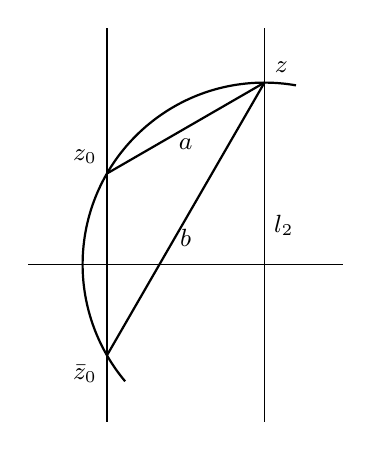
\begin{tikzpicture}
        \usetikzlibrary{calc}
        \draw (-5,0) -- (-1,0);
        \draw (-4,-2) -- (-4,3);
        \draw (-2,-2) --node[right]{\small\(l_2\)} (-2,3);
        \draw[thick] (-2,2.3094) arc (90:220:2.3094);
        \draw[thick] (-2,2.3094) arc (90:80:2.3094);
        \draw[thick] (-2,2.3094) node[above right]{\small\(z\)} --node[below]{\small\(a\)} (-4,1.1547) node[above left]{\small\(z_0\)};
        \draw[thick] (-2,2.3094) --node[below]{\small\(b\)} (-4,-1.1547) node [below left]{\small\(\bar z_0\)};
    \end{tikzpicture}
\end{figure}

这个问题接下来的步骤就交给读者补全.\marginpar{\footnotesize 这还是讲义中的一道习题不是吗.}

讲义中最后一个没有处理的问题是双曲平面上的等距变换.
\begin{theorem}[Poincar\'e, 1882]
    双曲平面\(\mathbb{H}^2\)上的等距变换具有形式
    \[
        f(z)=\frac{\alpha z+\beta}{\gamma z+\delta}.
    \]
    或
    \[
        f(z)=\frac{-\alpha\bar z+\beta}{-\gamma\bar z+\delta}
    \]
    其中\(\alpha,\beta,\gamma,\delta\in\mathbb{R}\)且\(\alpha\delta-\beta\gamma=1\). 第一种等距变换是保定向的; 第二种是反定向的.
\end{theorem}
\begin{proof}
    我们先证明所有这种形式的变换都是等距的. 对于\(f(z)=\frac{\alpha z+\beta}{\gamma z+\delta}\), 作如下变换.
    \begin{align*}
        f(z)&=\frac{\alpha z+\beta}{\gamma z+\delta}\\
            &=\frac{\alpha z+\frac{\alpha\delta}{\gamma}+\beta-\frac{\alpha\delta}{\gamma}}{\gamma z+\delta}\\
            &=\frac{\alpha}{\gamma}+\frac{\beta\gamma-\alpha\delta}{\gamma(\gamma z+\delta)}\\
            &=\frac{\alpha}{\gamma}-\frac{1}{\gamma(\gamma z+\delta)}.
    \end{align*}
    如果有\(f_{x_0}(z)=z+x_0,g_{\lambda}(z)=\lambda z,h(z)=-\frac{1}{z}\), 则\(f=f_{\alpha/\gamma}\circ h\circ g_\gamma\circ f_\delta\circ g_\gamma\). 既然每一项都是等距变换, \(f\)自然是等距变换. 第二种是将第一种复合关于\(y\)轴对称, 所以也是等距变换.

    另一方面, 与欧氏空间里一样, 我们用反射和三反射定理来刻画所有等距变换. 反射的选择是直观的, 即保持一条测地线不变的等距变换. 既然\(\mathbb{H}^2\)中测地线是圆弧, 反射自然地变成了关于此圆的反演, \(f(z)=\frac{\epsilon\bar z+\rho^2-\epsilon^2}{\bar z-\epsilon}\), 其中\(\epsilon\)是圆心, \(\rho\)是半径.
\begin{lemma}
    到两点\(z_1,z_2\)距离相等的点构成的集合是测地线, 关于此测地线的反射交换\(z_1,z_2\).
\end{lemma}
\begin{proof}
    任意测地线都可以通过等距变换变为\(y\)轴. 具体而言, 测地线\(x=x_0\)可以用平移\(f(z)=z-x_0\)变为\(y\)轴, 而测地线\((x-x_0)^2+y^2=r^2\)可以用关于圆\((x-x_0-r)^2+y^2=4r^2\)的反演变为\(x=x_0-r\).
    \begin{figure}[!ht]
        \centering
        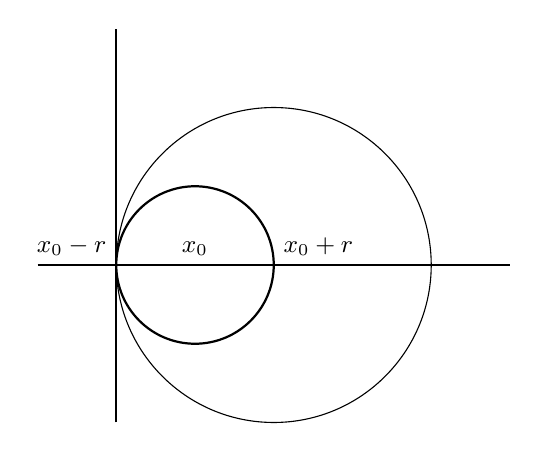
\begin{tikzpicture}
            \draw (0,0) -- (6,0);
            \draw[thick] (1,-2)--(1,3);
            \draw[thick] (2,0) circle [radius=1];
            \draw (3,0) circle [radius=2];
            \node[above] (A) at (2,0){\small\(x_0\)};
            \node[above right] (B) at (3,0){\small\(x_0+r\)};
            \node[above left] (C) at (1,0){\small\(x_0-r\)};
        \end{tikzpicture}
    \end{figure}

    所以我们不妨可设\(z_1,z_2\)关于\(y\)轴对称, 而关于\(y\)轴的反射\(r(z)=-\bar z\)将\(z_1,z_2\)映到对方, 且保持\(y\)轴上的点不变, 所以\(y\)轴上的点到\(z_1,z_2\)距离相同. 现假设还有另外的点\(w\)到\(z_1,z_2\)距离相同, 并考虑\(w'=r(w)\).
    \begin{figure}[!ht]
        \centering
        \begin{tikzpicture}
            \draw (0,0)--(0,5);
            \draw (-2,1) node[below]{\small\(z_1\)} arc (180:140:4);
            \draw (2,1) node[below]{\small\(z_2\)}arc (0:40:4);
            \draw[name path=circ1] (-2,1) arc (160:100:4);
            \draw[name path=circ2] (2,1) arc (20:80:4);
            \path[name intersections={of=circ1 and circ2}];
            \node[below left] (P) at (intersection-1){\small\(u\)};
            \node (A) at (-1,3.8){\small\(w\)};
            \node (B) at (1,3.8){\small\(w'\)};
        \end{tikzpicture}
    \end{figure}

    我们就有
    \[
        d(z_1,w)=d(z_2,w)=d(z_1,w')=d(z_1,u)+d(u,w')=d(z_1,u)+d(u,w).
    \]
    这与三角不等式矛盾, 而三角不等式是测地线的性质得到, 见第\ref{sec:3}节. 因此, 到\(z_1\)和\(z_2\)等距的点恰好是这条测地线.
\end{proof}
这样以来, 三反射定理的证明就可以完全参考欧式空间的版本, 不需要作什么改动了. 于是有
\begin{lemma}[\(\mathbb{H}^2\)上的三反射定理]\label{lem:1}
    每一个\(\mathbb{H}^2\)中的等距变换都可以拆分成一个, 两个或三个反射的复合.
\end{lemma}
回到原定理的证明. 既然反射就是关于测地线的反演, 有如下两种形式.
\begin{gather*}
    f(z)=\frac{\epsilon\bar z+\rho^2-\epsilon^2}{\bar z-\epsilon}=\frac{\lambda\bar z+1-\lambda^2}{\bar z-\lambda},\quad\lambda=\frac{\epsilon}{\rho}\\
    g(z)=2\epsilon-\bar z=\frac{-\bar z+2\epsilon}{1},
\end{gather*}
且都满足``\(\alpha\delta-\beta\gamma=1\)''的要求. 容易验证, 两个这种形式的变换的复合仍然是这种形式. 由引理\ref{lem:1}, 所有等距变换都可以表示成这种形式.
\end{proof}
\end{document}
